\documentclass[twoside]{book}

% Packages required by doxygen
\usepackage{calc}
\usepackage{doxygen}
\usepackage{graphicx}
\usepackage[utf8]{inputenc}
\usepackage{makeidx}
\usepackage{multicol}
\usepackage{multirow}
\usepackage{textcomp}
\usepackage[table]{xcolor}

% Font selection
\usepackage[T1]{fontenc}
\usepackage{mathptmx}
\usepackage[scaled=.90]{helvet}
\usepackage{courier}
\usepackage{amssymb}
\usepackage{sectsty}
\renewcommand{\familydefault}{\sfdefault}
\allsectionsfont{%
  \fontseries{bc}\selectfont%
  \color{darkgray}%
}
\renewcommand{\DoxyLabelFont}{%
  \fontseries{bc}\selectfont%
  \color{darkgray}%
}

% Page & text layout
\usepackage{geometry}
\geometry{%
  a4paper,%
  top=2.5cm,%
  bottom=2.5cm,%
  left=2.5cm,%
  right=2.5cm%
}
\tolerance=750
\hfuzz=15pt
\hbadness=750
\setlength{\emergencystretch}{15pt}
\setlength{\parindent}{0cm}
\setlength{\parskip}{0.2cm}
\makeatletter
\renewcommand{\paragraph}{%
  \@startsection{paragraph}{4}{0ex}{-1.0ex}{1.0ex}{%
    \normalfont\normalsize\bfseries\SS@parafont%
  }%
}
\renewcommand{\subparagraph}{%
  \@startsection{subparagraph}{5}{0ex}{-1.0ex}{1.0ex}{%
    \normalfont\normalsize\bfseries\SS@subparafont%
  }%
}
\makeatother

% Headers & footers
\usepackage{fancyhdr}
\pagestyle{fancyplain}
\fancyhead[LE]{\fancyplain{}{\bfseries\thepage}}
\fancyhead[CE]{\fancyplain{}{}}
\fancyhead[RE]{\fancyplain{}{\bfseries\leftmark}}
\fancyhead[LO]{\fancyplain{}{\bfseries\rightmark}}
\fancyhead[CO]{\fancyplain{}{}}
\fancyhead[RO]{\fancyplain{}{\bfseries\thepage}}
\fancyfoot[LE]{\fancyplain{}{}}
\fancyfoot[CE]{\fancyplain{}{}}
\fancyfoot[RE]{\fancyplain{}{\bfseries\scriptsize Generated on Fri Nov 29 2013 15\-:18\-:56 for Chu\-Thread by Doxygen }}
\fancyfoot[LO]{\fancyplain{}{\bfseries\scriptsize Generated on Fri Nov 29 2013 15\-:18\-:56 for Chu\-Thread by Doxygen }}
\fancyfoot[CO]{\fancyplain{}{}}
\fancyfoot[RO]{\fancyplain{}{}}
\renewcommand{\footrulewidth}{0.4pt}
\renewcommand{\chaptermark}[1]{%
  \markboth{#1}{}%
}
\renewcommand{\sectionmark}[1]{%
  \markright{\thesection\ #1}%
}

% Indices & bibliography
\usepackage{natbib}
\usepackage[titles]{tocloft}
\setcounter{tocdepth}{3}
\setcounter{secnumdepth}{5}
\makeindex

% Hyperlinks (required, but should be loaded last)
\usepackage{ifpdf}
\ifpdf
  \usepackage[pdftex,pagebackref=true]{hyperref}
\else
  \usepackage[ps2pdf,pagebackref=true]{hyperref}
\fi
\hypersetup{%
  colorlinks=true,%
  linkcolor=blue,%
  citecolor=blue,%
  unicode%
}

% Custom commands
\newcommand{\clearemptydoublepage}{%
  \newpage{\pagestyle{empty}\cleardoublepage}%
}


%===== C O N T E N T S =====

\begin{document}

% Titlepage & ToC
\hypersetup{pageanchor=false}
\pagenumbering{roman}
\begin{titlepage}
\vspace*{7cm}
\begin{center}%
{\Large Chu\-Thread }\\
\vspace*{1cm}
{\large Generated by Doxygen 1.8.5}\\
\vspace*{0.5cm}
{\small Fri Nov 29 2013 15:18:56}\\
\end{center}
\end{titlepage}
\clearemptydoublepage
\tableofcontents
\clearemptydoublepage
\pagenumbering{arabic}
\hypersetup{pageanchor=true}

%--- Begin generated contents ---
\chapter{Bug List}
\label{bug}
\hypertarget{bug}{}

\begin{DoxyRefList}
\item[\label{bug__bug000001}%
\hypertarget{bug__bug000001}{}%
File \hyperlink{_chu_thread_8h}{Chu\-Thread.h} ]Currently no bug found yet
\end{DoxyRefList}
\chapter{Hierarchical Index}
\section{Class Hierarchy}
This inheritance list is sorted roughly, but not completely, alphabetically\-:\begin{DoxyCompactList}
\item \contentsline{section}{chu\-Thread\-Namespace\-:\-:Chu\-Thread$<$ T1, T2 $>$}{\pageref{classchu_thread_namespace_1_1_chu_thread}}{}
\item \contentsline{section}{chu\-Thread\-Namespace\-:\-:Chu\-Thread$<$ Sturct, Sturct $>$}{\pageref{classchu_thread_namespace_1_1_chu_thread}}{}
\begin{DoxyCompactList}
\item \contentsline{section}{My\-Thread}{\pageref{class_my_thread}}{}
\end{DoxyCompactList}
\item \contentsline{section}{Sturct}{\pageref{struct_sturct}}{}
\end{DoxyCompactList}

\chapter{Class Index}
\section{Class List}
Here are the classes, structs, unions and interfaces with brief descriptions\-:\begin{DoxyCompactList}
\item\contentsline{section}{\hyperlink{classchu_thread_namespace_1_1_chu_thread}{chu\-Thread\-Namespace\-::\-Chu\-Thread$<$ T1, T2 $>$} }{\pageref{classchu_thread_namespace_1_1_chu_thread}}{}
\item\contentsline{section}{\hyperlink{class_my_thread}{My\-Thread} }{\pageref{class_my_thread}}{}
\item\contentsline{section}{\hyperlink{struct_sturct}{Sturct} }{\pageref{struct_sturct}}{}
\end{DoxyCompactList}

\chapter{File Index}
\section{File List}
Here is a list of all documented files with brief descriptions\-:\begin{DoxyCompactList}
\item\contentsline{section}{D\-:/\-Dropbox/\-Programing/\-Chu\-Thread/thread/\hyperlink{_chu_thread_8h}{Chu\-Thread.\-h} \\*This is a windows thread class, and it can be inherited by other class which needs multi-\/thread fucntion }{\pageref{_chu_thread_8h}}{}
\end{DoxyCompactList}

\chapter{Class Documentation}
\hypertarget{classchu_thread_namespace_1_1_chu_thread}{\section{chu\-Thread\-Namespace\-:\-:Chu\-Thread$<$ T1, T2 $>$ Class Template Reference}
\label{classchu_thread_namespace_1_1_chu_thread}\index{chu\-Thread\-Namespace\-::\-Chu\-Thread$<$ T1, T2 $>$@{chu\-Thread\-Namespace\-::\-Chu\-Thread$<$ T1, T2 $>$}}
}
\subsection*{Public Member Functions}
\begin{DoxyCompactItemize}
\item 
\hyperlink{classchu_thread_namespace_1_1_chu_thread_a9fc3a821c0969a7dcaaf5b4e9c62365c}{Chu\-Thread} ()
\item 
void \hyperlink{classchu_thread_namespace_1_1_chu_thread_a0c9ac5b4b19ae1ce58f14dc180f845ad}{start\-Thread} ()
\item 
virtual void \hyperlink{classchu_thread_namespace_1_1_chu_thread_a3043a3b3a99b5e96a0ce2e4591fdb0cf}{thread} ()
\item 
\hypertarget{classchu_thread_namespace_1_1_chu_thread_a910489dcf014618f45c7091f9df8454c}{void {\bfseries set\-Local\-Variable} (T1 arg)}\label{classchu_thread_namespace_1_1_chu_thread_a910489dcf014618f45c7091f9df8454c}

\item 
\hypertarget{classchu_thread_namespace_1_1_chu_thread_a3b5dc1ef661f2f796f21b5201bcd962a}{const T1 {\bfseries get\-Local\-Variable} ()}\label{classchu_thread_namespace_1_1_chu_thread_a3b5dc1ef661f2f796f21b5201bcd962a}

\item 
void \hyperlink{classchu_thread_namespace_1_1_chu_thread_a263626e9fbb344f14da6f30e7b277639}{set\-Share\-Variable} (T2 arg)
\item 
const T2 \hyperlink{classchu_thread_namespace_1_1_chu_thread_a611c714a581e0c07b73b0680564ba866}{get\-Share\-Variable} ()
\item 
\hypertarget{classchu_thread_namespace_1_1_chu_thread_adf36076d451d88a938af87e2f6172b9d}{void {\bfseries set\-Interrupt\-Flag} ()}\label{classchu_thread_namespace_1_1_chu_thread_adf36076d451d88a938af87e2f6172b9d}

\item 
bool \hyperlink{classchu_thread_namespace_1_1_chu_thread_a67c6c5e21f2aa7ba25e00cba05987cc6}{stop\-Current\-Thread} ()
\end{DoxyCompactItemize}
\subsection*{Protected Attributes}
\begin{DoxyCompactItemize}
\item 
\hypertarget{classchu_thread_namespace_1_1_chu_thread_aa7f6bfbab64f35aa66cc535ee6dee5e0}{H\-A\-N\-D\-L\-E {\bfseries localhot\-H\-A\-N\-D\-L\-E}}\label{classchu_thread_namespace_1_1_chu_thread_aa7f6bfbab64f35aa66cc535ee6dee5e0}

\end{DoxyCompactItemize}


\subsection{Constructor \& Destructor Documentation}
\hypertarget{classchu_thread_namespace_1_1_chu_thread_a9fc3a821c0969a7dcaaf5b4e9c62365c}{\index{chu\-Thread\-Namespace\-::\-Chu\-Thread@{chu\-Thread\-Namespace\-::\-Chu\-Thread}!Chu\-Thread@{Chu\-Thread}}
\index{Chu\-Thread@{Chu\-Thread}!chuThreadNamespace::ChuThread@{chu\-Thread\-Namespace\-::\-Chu\-Thread}}
\subsubsection[{Chu\-Thread}]{\setlength{\rightskip}{0pt plus 5cm}template$<$class T1 , class T2 $>$ {\bf chu\-Thread\-Namespace\-::\-Chu\-Thread}$<$ T1, T2 $>$\-::{\bf Chu\-Thread} (
\begin{DoxyParamCaption}
{}
\end{DoxyParamCaption}
)}}\label{classchu_thread_namespace_1_1_chu_thread_a9fc3a821c0969a7dcaaf5b4e9c62365c}
Function Name\-: Constructor Function Purpose\-: Do noting 

\subsection{Member Function Documentation}
\hypertarget{classchu_thread_namespace_1_1_chu_thread_a611c714a581e0c07b73b0680564ba866}{\index{chu\-Thread\-Namespace\-::\-Chu\-Thread@{chu\-Thread\-Namespace\-::\-Chu\-Thread}!get\-Share\-Variable@{get\-Share\-Variable}}
\index{get\-Share\-Variable@{get\-Share\-Variable}!chuThreadNamespace::ChuThread@{chu\-Thread\-Namespace\-::\-Chu\-Thread}}
\subsubsection[{get\-Share\-Variable}]{\setlength{\rightskip}{0pt plus 5cm}template$<$class T1 , class T2 $>$ const T2 {\bf chu\-Thread\-Namespace\-::\-Chu\-Thread}$<$ T1, T2 $>$\-::get\-Share\-Variable (
\begin{DoxyParamCaption}
{}
\end{DoxyParamCaption}
)}}\label{classchu_thread_namespace_1_1_chu_thread_a611c714a581e0c07b73b0680564ba866}
Function Name\-: get\-Share\-Variable Function Purpose\-: Get the static global variabel and return \hypertarget{classchu_thread_namespace_1_1_chu_thread_a263626e9fbb344f14da6f30e7b277639}{\index{chu\-Thread\-Namespace\-::\-Chu\-Thread@{chu\-Thread\-Namespace\-::\-Chu\-Thread}!set\-Share\-Variable@{set\-Share\-Variable}}
\index{set\-Share\-Variable@{set\-Share\-Variable}!chuThreadNamespace::ChuThread@{chu\-Thread\-Namespace\-::\-Chu\-Thread}}
\subsubsection[{set\-Share\-Variable}]{\setlength{\rightskip}{0pt plus 5cm}template$<$class T1 , class T2$>$ void {\bf chu\-Thread\-Namespace\-::\-Chu\-Thread}$<$ T1, T2 $>$\-::set\-Share\-Variable (
\begin{DoxyParamCaption}
\item[{T2}]{arg}
\end{DoxyParamCaption}
)}}\label{classchu_thread_namespace_1_1_chu_thread_a263626e9fbb344f14da6f30e7b277639}
Function Name\-: set\-Share\-Variable Function Purpose\-: Set the global variabel to a static class variable for all thread access \hypertarget{classchu_thread_namespace_1_1_chu_thread_a0c9ac5b4b19ae1ce58f14dc180f845ad}{\index{chu\-Thread\-Namespace\-::\-Chu\-Thread@{chu\-Thread\-Namespace\-::\-Chu\-Thread}!start\-Thread@{start\-Thread}}
\index{start\-Thread@{start\-Thread}!chuThreadNamespace::ChuThread@{chu\-Thread\-Namespace\-::\-Chu\-Thread}}
\subsubsection[{start\-Thread}]{\setlength{\rightskip}{0pt plus 5cm}template$<$class T1 , class T2 $>$ void {\bf chu\-Thread\-Namespace\-::\-Chu\-Thread}$<$ T1, T2 $>$\-::start\-Thread (
\begin{DoxyParamCaption}
{}
\end{DoxyParamCaption}
)}}\label{classchu_thread_namespace_1_1_chu_thread_a0c9ac5b4b19ae1ce58f14dc180f845ad}
Function Name\-: start\-Thread Function Purpose\-: Create an other thread to execute open\-Thread function by W\-I\-N\-\_\-\-A\-P\-I \hypertarget{classchu_thread_namespace_1_1_chu_thread_a67c6c5e21f2aa7ba25e00cba05987cc6}{\index{chu\-Thread\-Namespace\-::\-Chu\-Thread@{chu\-Thread\-Namespace\-::\-Chu\-Thread}!stop\-Current\-Thread@{stop\-Current\-Thread}}
\index{stop\-Current\-Thread@{stop\-Current\-Thread}!chuThreadNamespace::ChuThread@{chu\-Thread\-Namespace\-::\-Chu\-Thread}}
\subsubsection[{stop\-Current\-Thread}]{\setlength{\rightskip}{0pt plus 5cm}template$<$class T1 , class T2 $>$ bool {\bf chu\-Thread\-Namespace\-::\-Chu\-Thread}$<$ T1, T2 $>$\-::stop\-Current\-Thread (
\begin{DoxyParamCaption}
{}
\end{DoxyParamCaption}
)}}\label{classchu_thread_namespace_1_1_chu_thread_a67c6c5e21f2aa7ba25e00cba05987cc6}
Function Name\-: start\-Thread Function Purpose\-: Create an other thread to execute open\-Thread function by W\-I\-N\-\_\-\-A\-P\-I \hypertarget{classchu_thread_namespace_1_1_chu_thread_a3043a3b3a99b5e96a0ce2e4591fdb0cf}{\index{chu\-Thread\-Namespace\-::\-Chu\-Thread@{chu\-Thread\-Namespace\-::\-Chu\-Thread}!thread@{thread}}
\index{thread@{thread}!chuThreadNamespace::ChuThread@{chu\-Thread\-Namespace\-::\-Chu\-Thread}}
\subsubsection[{thread}]{\setlength{\rightskip}{0pt plus 5cm}template$<$class T1 , class T2 $>$ void {\bf chu\-Thread\-Namespace\-::\-Chu\-Thread}$<$ T1, T2 $>$\-::thread (
\begin{DoxyParamCaption}
{}
\end{DoxyParamCaption}
)\hspace{0.3cm}{\ttfamily [virtual]}}}\label{classchu_thread_namespace_1_1_chu_thread_a3043a3b3a99b5e96a0ce2e4591fdb0cf}
Function Name\-: thread Function Purpose\-: The fucntion will be overrided by thread and run in multi-\/thread 

The documentation for this class was generated from the following files\-:\begin{DoxyCompactItemize}
\item 
D\-:/\-Dropbox/\-Programing/\-Chu\-Thread/thread/\hyperlink{_chu_thread_8h}{Chu\-Thread.\-h}\item 
D\-:/\-Dropbox/\-Programing/\-Chu\-Thread/thread/Chu\-Thread.\-cpp\end{DoxyCompactItemize}

\hypertarget{class_my_thread}{\section{My\-Thread Class Reference}
\label{class_my_thread}\index{My\-Thread@{My\-Thread}}
}
Inheritance diagram for My\-Thread\-:\begin{figure}[H]
\begin{center}
\leavevmode
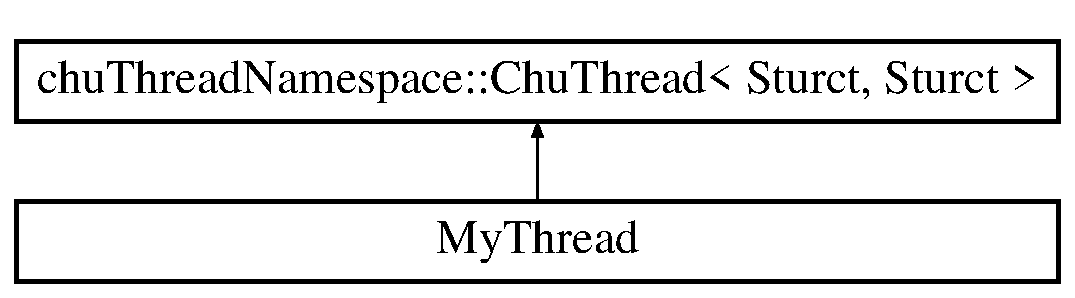
\includegraphics[height=2.000000cm]{class_my_thread}
\end{center}
\end{figure}
\subsection*{Additional Inherited Members}


The documentation for this class was generated from the following file\-:\begin{DoxyCompactItemize}
\item 
D\-:/\-Dropbox/\-Programing/\-Chu\-Thread/thread/main.\-cpp\end{DoxyCompactItemize}

\hypertarget{struct_sturct}{\section{Sturct Struct Reference}
\label{struct_sturct}\index{Sturct@{Sturct}}
}
\subsection*{Public Attributes}
\begin{DoxyCompactItemize}
\item 
\hypertarget{struct_sturct_ac8ad5e343771985d2db1abb51f32848a}{int {\bfseries int\-Data}}\label{struct_sturct_ac8ad5e343771985d2db1abb51f32848a}

\item 
\hypertarget{struct_sturct_a50f54d847a3e8674472a3ae6433e878e}{double {\bfseries double\-Data}}\label{struct_sturct_a50f54d847a3e8674472a3ae6433e878e}

\end{DoxyCompactItemize}


The documentation for this struct was generated from the following file\-:\begin{DoxyCompactItemize}
\item 
D\-:/\-Dropbox/\-Programing/\-Chu\-Thread/thread/main.\-cpp\end{DoxyCompactItemize}

\chapter{File Documentation}
\hypertarget{_chu_thread_8h}{\section{D\-:/\-Dropbox/\-Programing/\-Chu\-Thread/thread/\-Chu\-Thread.h File Reference}
\label{_chu_thread_8h}\index{D\-:/\-Dropbox/\-Programing/\-Chu\-Thread/thread/\-Chu\-Thread.\-h@{D\-:/\-Dropbox/\-Programing/\-Chu\-Thread/thread/\-Chu\-Thread.\-h}}
}


This is a windows thread class, and it can be inherited by other class which needs multi-\/thread fucntion.  


{\ttfamily \#include $<$iostream$>$}\\*
{\ttfamily \#include $<$vector$>$}\\*
{\ttfamily \#include \char`\"{}windows.\-h\char`\"{}}\\*
{\ttfamily \#include \char`\"{}process.\-h\char`\"{}}\\*
\subsection*{Classes}
\begin{DoxyCompactItemize}
\item 
class \hyperlink{classchu_thread_namespace_1_1_chu_thread}{chu\-Thread\-Namespace\-::\-Chu\-Thread$<$ T1, T2 $>$}
\end{DoxyCompactItemize}


\subsection{Detailed Description}
This is a windows thread class, and it can be inherited by other class which needs multi-\/thread fucntion. \begin{DoxyAuthor}{Authors}
Ting-\/\-Sheng Chu 
\end{DoxyAuthor}
\begin{DoxyVersion}{Version}
1.\-0 
\end{DoxyVersion}
\begin{DoxyDate}{Date}
2013-\/11 
\end{DoxyDate}
\begin{DoxyCopyright}{Copyright}
G\-N\-U Public License.
\end{DoxyCopyright}
\begin{DoxyPrecond}{Precondition}
Windows\-\_\-\-A\-P\-I 
\end{DoxyPrecond}
\begin{DoxyRefDesc}{Bug}
\item[\hyperlink{bug__bug000001}{Bug}]Currently no bug found yet\end{DoxyRefDesc}
\hypertarget{_chu_thread_8h_Revise_Log}{}\subsection{Revise\-\_\-\-Log}\label{_chu_thread_8h_Revise_Log}
13/11/20 Add the close thread function \par

%--- End generated contents ---

% Index
\newpage
\phantomsection
\addcontentsline{toc}{part}{Index}
\printindex

\end{document}
